\dev{Emile Martiez}{}

\begin{definition}
	$$lev(w_1, w_2) = \min \left\{k \in \N \big/ \exists f_1, \dots, f_k \in \{ins_{a,i}, sub_{a,i}, sup_i / a\in \Sigma, i\in \N\} \: : \: w_2 = f_k \circ \dots \circ f_1 (w_1)\right\}$$
\end{definition}

\begin{proposition}
	$$
	\begin{array}{rl}
		lev(u, \epsilon) = & |u|\\
		lev(\epsilon, v) = & |v|\\
		lev(u.a, v.b) = & \min \left\{ \begin{array}{ll}
			lev(u,v) + 1 \quad & \text{sub}\\
			lev(u.a, v) + 1 & \text{ins}\\
			lev(u, v.b) + 1 & \text{sup}\\
			lev(u, v) & \text{si } a = b
		\end{array}\right.
	\end{array}$$
\end{proposition}


\paragraph{Idee} On peut commencer par la dernière lettre, et alors appliquer une des transformations possibles. Mettons cette idée en preuve.

\paragraph{Notation} Pour $f \in \{ins_{a,i}, sub_{a,i}, sup_i\}$, notons $i = \alpha(f)$.

\begin{lemma}
	Pour $u,v\in \Sigma^*$, avec $k = lev(u,v)$, il existe une transformation minimale $f_k \circ \dots \circ f_1$ avec $\alpha(f_j) \leq \alpha(f_{j-1})$ avec égalité seulement si $f_{j} = ins$
\end{lemma}

\paragraph{Intuition} On peut traiter les lettres dans l'ordre, et une fois chacune.\\
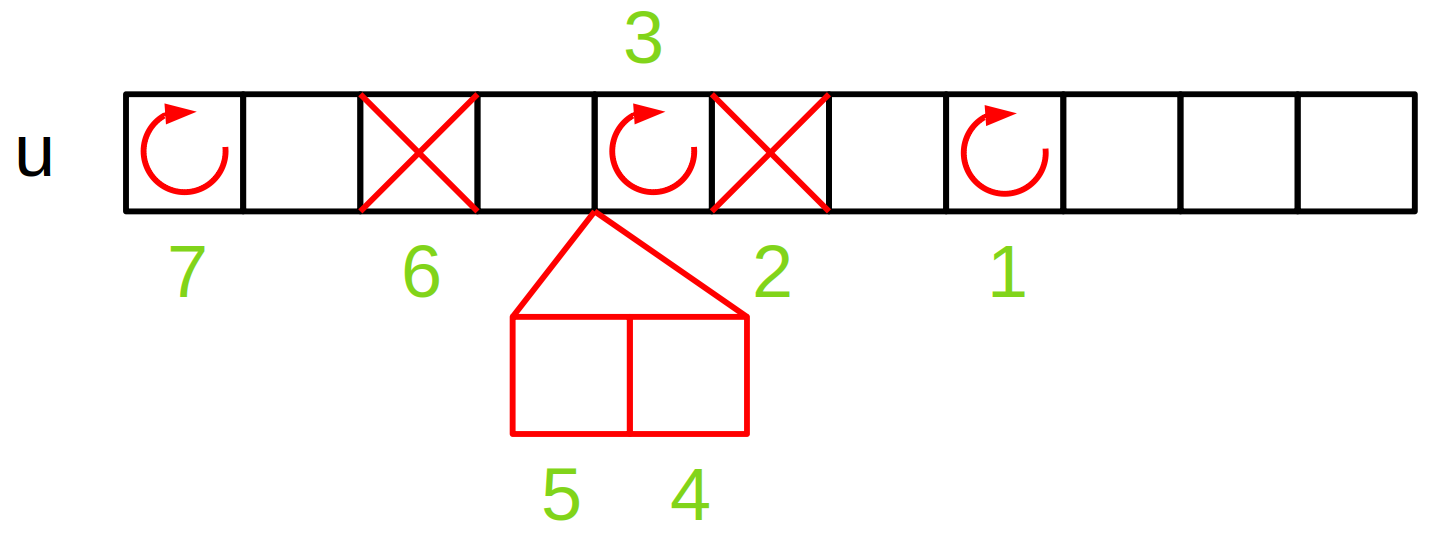
\includegraphics[width = 0.7\linewidth]{nouveau_dev/levenstein/tri_operation.png}

\begin{proof}
	Intution de la preuve : On fait des inversions comme pour un tri à bulle.\\
	
	Tant qu'il reste $j$ne vérifiant pas la condition, alors on échange $f_j$ et $f_{j-1}$. Par exemple : si $f_j = ins_{b, i1}$ et $f_{j-1} = sup_{i_2}$ avec donc $i_1 > i_2$ (on est dans le cas d'égalité sinon), alors $f_j \circ f_{j-1} = sup_{i_2} \circ ins_{b, i_1+1}$.\\
	Les seuls cas où l'on ne peut pas inverser sont ceux ou la même lettre est concerné (ex : $sup_i \circ ins_i$) mais qui sont interdits par minimalité.\\
	De plus, nos transformations termineront car les indices ne concernent que des lettres valides et ne font que croire.
\end{proof}

\begin{com}
	Ne pas hésiter à montrer les inversions et les différents cas sur le dessin.
\end{com}


\paragraph{Retour sur la propriété} Montrons maintenant par induction que nous calculons la bonne distance. \\
\begin{proof}
	\begin{itemize}[label = $\star$]
		\item Si $u = \epsilon$ ou si $v = \epsilon$, alors on ne peut en effet pas faire mieux que $|v|$ insertions ou $|u|$ suppressions.
		\item On prend une transformation minimale $f_k \circ \dots f_1$ du lemme. Alors \begin{itemize}[label = $\bullet$]
			\item Soit $\alpha(f_1) < |u|$ et alors, comme on on ne pourra jamais toucher de lettre plus loin que $f_1$, $a = b$, et la transformation restante est minimale pour $u, v$ (sinon on pourrait en faire une plus petite pour $u.a, v.b$), d'où le résultat par hypothèse d'induction 
			\item Soit $\alpha(f_1) = |u|$ et alors il fait soit une suppression (ce que l'on gère), soit une substitution (resp. une insertion). Il ne peut alors que mettre la lettre $b$ (car on ne rechangera rien après $b$). Ainsi on a bien la mise de $b$, puis une transformation de $u$ en $v$ (resp. de $u.a$ en $v$) (car on ne retouchera aucune lettre après $b$). Or cette transformation est minimale car sinon on aurait pu faire mieux. D'où le résultat par hypothèse d'induction.
		\end{itemize}
	\end{itemize}
	\begin{com}
		On ne montre ici que l'inégalité difficile, mais on obtient la facile en disant que ce qu'on fait sinon c'est quand meme des transformations, donc elle ne font pas mieux que le minimum.
	\end{com}

\end{proof}

\textit{Bon la du coup on montrait le tableau qu'on prend, la complexité, et tout le tin touin. A voir ce qu'on récupère de Malloy pour le mettre ici}